% coding:utf-8

%FOSASTOC, a LaTeX-Code for a electrical summary of stochastic
%Copyright (C) 2013, Daniel Winz, Ervin Mazlagic

%This program is free software; you can redistribute it and/or
%modify it under the terms of the GNU General Public License
%as published by the Free Software Foundation; either version 2
%of the License, or (at your option) any later version.

%This program is distributed in the hope that it will be useful,
%but WITHOUT ANY WARRANTY; without even the implied warranty of
%MERCHANTABILITY or FITNESS FOR A PARTICULAR PURPOSE.  See the
%GNU General Public License for more details.
%----------------------------------------

\chapter{Diskrete Verteilungen}
Diskrete Verteilungen beschreiben Probleme, welche
Ergebnisse aus $\mathbb{N}$ liefern und binär sind.

\paragraph{Binär}
Binär bedeutet, dass ein Ereignis zwei Werte annehmen kann. Bekannte
Beispiele binärer Probleme sind
\begin{itemize}
	\item Gewinnlose \hfill{} (\emph{Gewinn, Zonk})
	\item Münzwurf \hfill{} (\emph{Kopf, Zahl})
	\item Telefon \hfill{} (\emph{klingelt, klingelt nicht})
\end{itemize}
Viele nicht-binäre Probleme können aber leicht in binäre gewandelt
werden. Beispielsweise liefert ein Sensor analoge Signale, diese sind
$\notin \mathbb{N}$ noch sind diese binär. 
Dennoch kann man das Signal binär
untersuchen mit der Fragestellung 
"`\emph{Ist der Wert grösser als $xy$?}"'.
Diese Frage kann semantisch nur mit \emph{Ja} und \emph{Nein} beantwortet
werden und beschreibt somit ein binäres Problem. Die Zahl der Antworten
kann wiederum nur $\in \mathbb{N}$ sein. Somit sind die Bedingungen 
für ein binäres Problem gegeben.

\newpage
\section{Hypergeometrische Verteilung}
Die hypergeometrische Verteilung entspricht dem Urnenmodell:
\begin{itemize}
	\item Urne hat $m$ rote (postive) und $n$ blaue (negative)
		Kugeln
		\[ m,n \in \mathbb{N} \]
	\item Die Menge der roten als auch der blauen Kugeln ist fix 
		\[ m,n \neq \infty \]
	\item Ein erzieltes Ergebnis reduziert die entsprechende Menge
		\[ m \rightarrow  M - 1\]
		Oft wird hier der Ausdruck \emph{Ziehen ohne Zurücklegen}
		verwendet.
\end{itemize}
Die hypergeometrische Verteilung wird im allgemeinen beschrieben mit
\[  
	X \sim Hyp(n,r,s)
\]
\[ \begin{array}{c l}
	n & \text{Anzahl Ziehungen} \\
	r & \text{Anzhal roter Kugeln} \\
	s & \text{Anzahl blauer Kugeln}
\end{array} \]


\subsection{Beispiel einer hypogeometrischen Verteilung}
Ein Beispiel aus dem Alltag ist die Teambildung im Mannschaftssport.
Ein Turnverein hat $9$ männliche und $17$ weibliche Mitglieder. Für ein
Fussballmatch gegen einen anderen Verein muss nun ein Team mit $11$
Mitgliedern gebildet werden. Wie wahrscheinlich ist es, dass das
Team aus einer bestimmten Anzahl Männern oder Frauen besteht?
\begin{Schunk}
\begin{Sinput}
> man <- 9; women <- 17; player <- 11
> boys <- dhyper(x=c(1:player), m=man, n=women, k=player)
> girls <- dhyper(x=(1:player), m=women, n=man, k=player)
> plot(boys, type='h')
> plot(girls, type='h')
\end{Sinput}
\end{Schunk}
\begin{figure}[h!]
\centering
\begin{subfigure}[b]{0.48\textwidth}
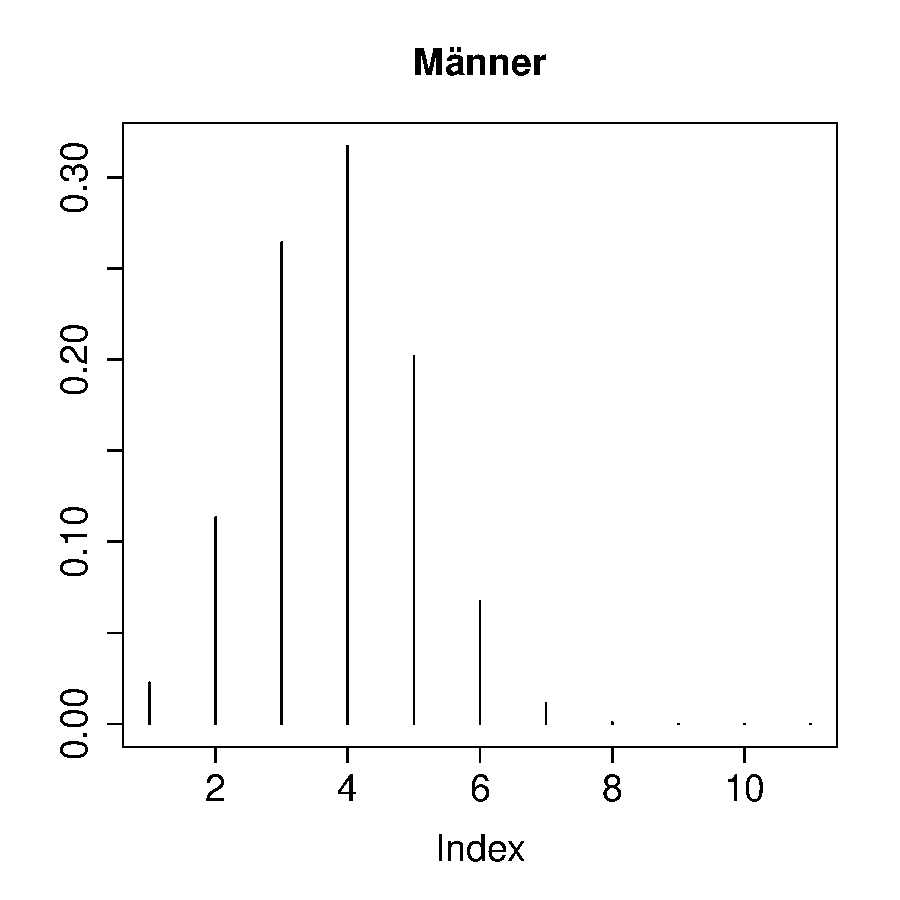
\includegraphics{verteilungen-004}
\caption{$P(x)$ der Männer im Team}
\end{subfigure}
\begin{subfigure}[b]{0.48\textwidth}
\centering
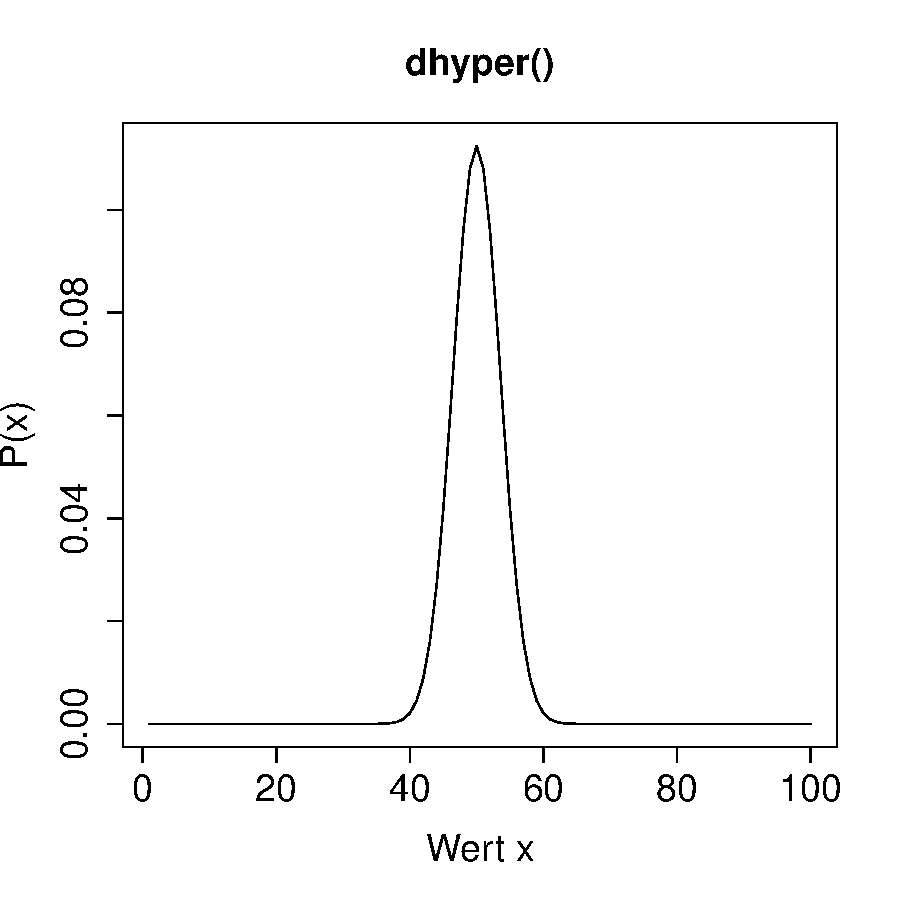
\includegraphics{verteilungen-005}
\caption{$P(x)$ der Frauen im Team}
\end{subfigure}
\caption{Teambildung nach Geschlecht}
\label{fig:team}
\end{figure}

\noindent
Die Plots aus der Abbildung \ref{fig:team} zeigen, dass es mit der 
höchsten Wahrscheinlichkeit
4 Männer und 7 Frauen im Team hat, was die gewünschte Anzahl von Spielern
ergibt für das Team ($4+7=11$). 

\clearpage
\newpage
\section{Binomialverteilung}
Die Binomialverteilung ist eine Verteilung, welche bei binären Problemen
auftritt wobei ein erzieltes Ergebnis nicht die weiteren Ergebnisse
beeinflusst. Sie ist somit ein Grenzfall der hypergeometrischen 
Verteilung (nämlich dann, wenn es sehr viele rote und blaue 
Kugeln gibt).
\[ 
	\lim_{r,s \rightarrow \infty} Hyp(n,r,s) 
	\quad \Rightarrow \quad Bin(n,p)
\]
\[ 
	X \sim Bin(n,p)
\]
\[ \begin{array}{c l} 
	n & \text{Anzahl Versuche} \\
	p & \text{Trefferwahrscheinlichkeit}
\end{array} \]

\subsection{Verwendung in R}
\lstinline{R} stellt grundsätzlich vier Funktionen für die 
Binomialverteilung zur Verfügung. 
\begin{itemize}
	\item \lstinline{dbinom()} \hfill{} 
		(\emph{Wahrscheinlichkeitsverteilung})
	\item \lstinline{pbinom()} \hfill{}
		(\emph{kumulative Wahrscheinlichkeit})
	\item \lstinline{qbinom()} \hfill{}
		(\emph{Verteilung der Quantile})
	\item \lstinline{rbinom()} \hfill{}
		(\emph{Zufallszahlen})
\end{itemize}
Die Abbildung \ref{fig:binom} zeigt jeweils einen Plot zu den gegebenen
Funktionen aus \lstinline{R}. Für weitere Informationen zu Plots siehe
Kapitel \ref{chap:plots}.





\begin{figure}[h!]
\centering
\begin{subfigure}[b]{0.48\textwidth}
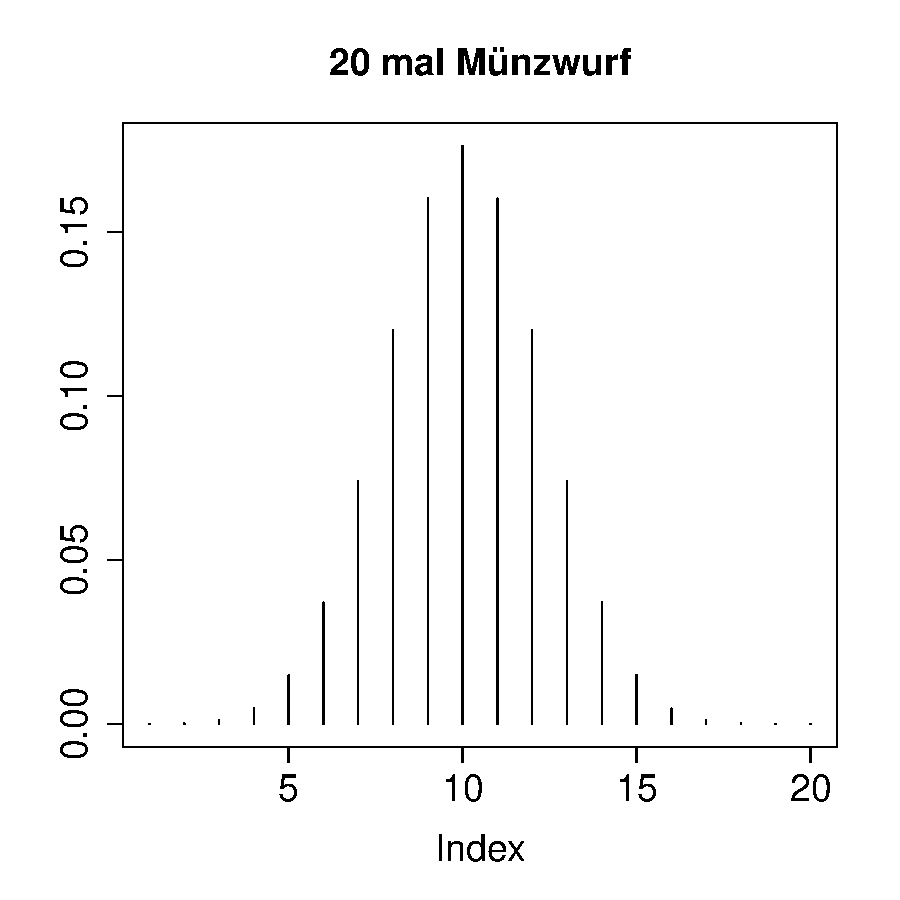
\includegraphics{verteilungen-010}
\caption{W.-Verteilung}
\end{subfigure}
\begin{subfigure}[b]{0.48\textwidth}
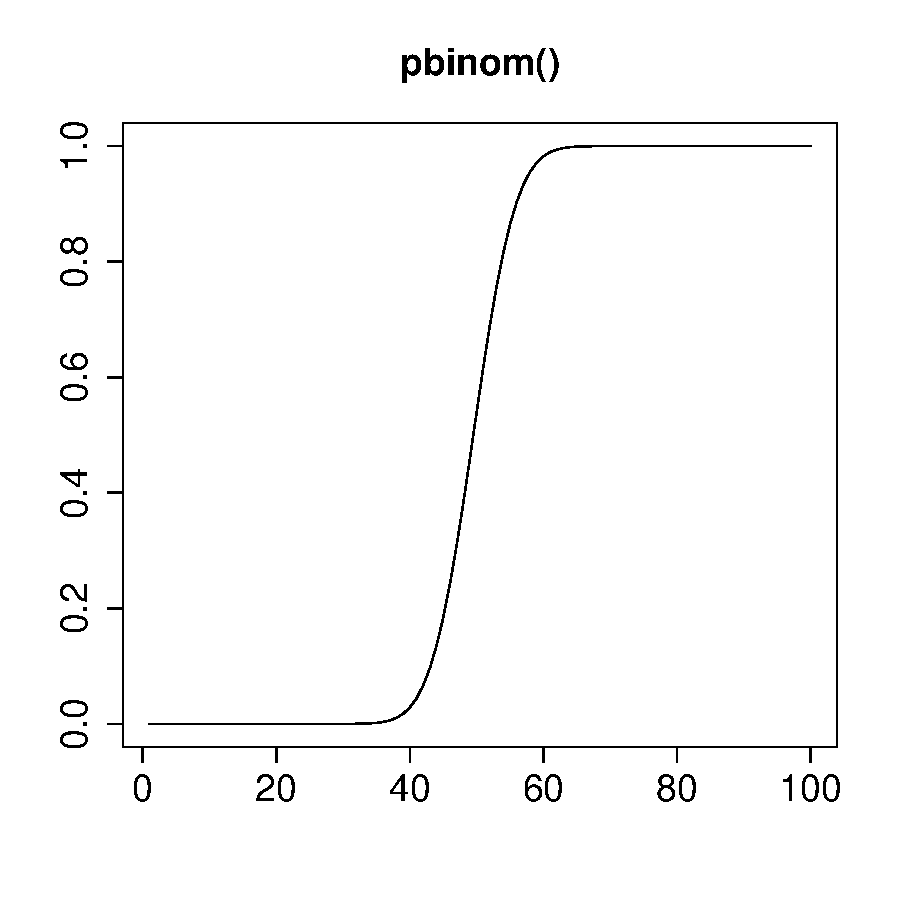
\includegraphics{verteilungen-011}
\caption{kumulative Wahrscheinlichkeit}
\end{subfigure}

\begin{subfigure}[b]{0.48\textwidth}
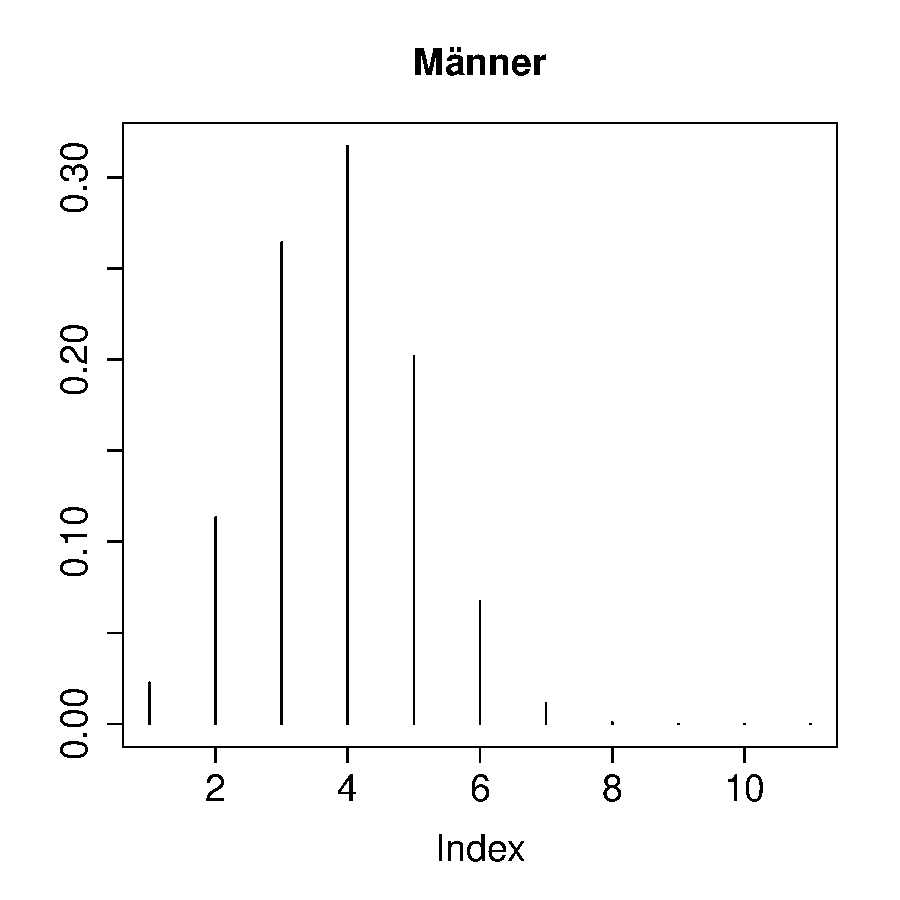
\includegraphics{verteilungen-012}
\caption{Quantile}
\end{subfigure}
\begin{subfigure}[b]{0.48\textwidth}
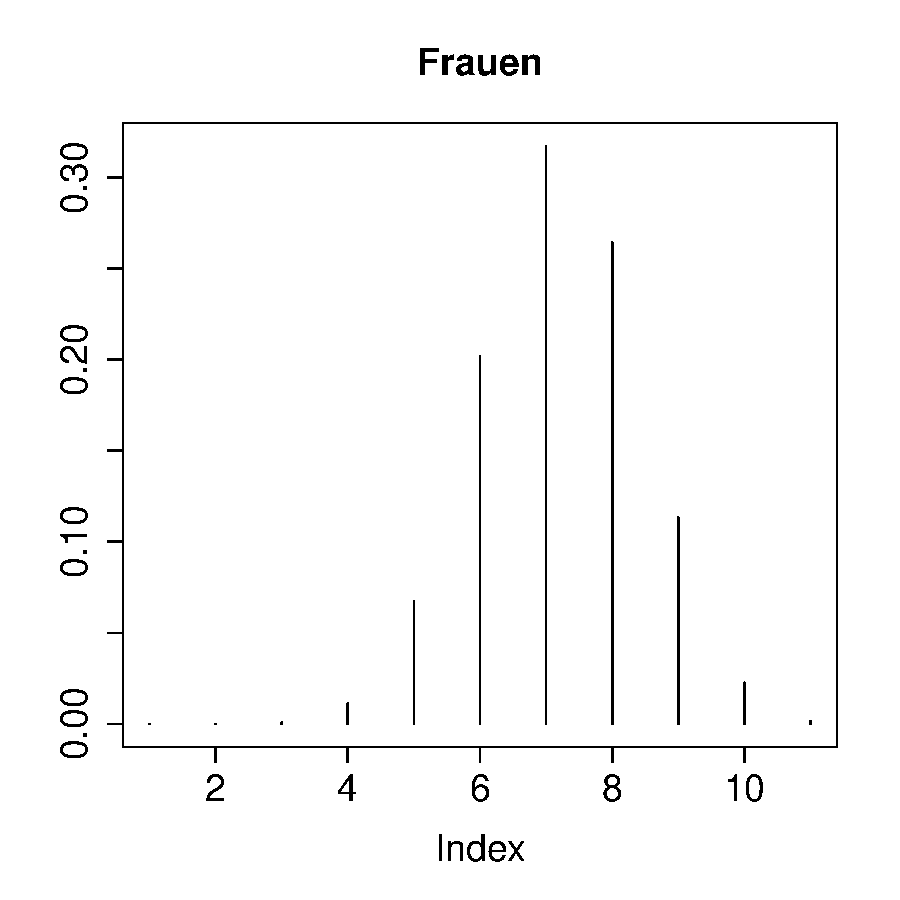
\includegraphics{verteilungen-013}
\caption{Zufallszahlen}
\end{subfigure}
\caption{Binomialverteilung ($n=100, p=0.5$)}
\label{fig:binom}
\end{figure}

\subsection{Beispiel einer binomialen Verteilung}
Jemand sagt Ihnen, dass er von 100 Münzwürfen 80 mal Kopf erhielt.
Sie antworten spontan, dass Sie ihm 15 Treffer von 20 Versuchen ja 
noch geglaubt hätten aber nicht 80 von 100. 
Wie wahrscheinlich sind aber diese beiden Ergebnisse wenn Kopf 
und Zahl jeweils gleichwahrscheinliche Ergebnisse sind?

\begin{Schunk}
\begin{Sinput}
> plot(dbinom(x=c(1:100), size=100, prob=0.5), type='h')
> plot(dbinom(x=c(1:20), size=20, prob=0.5), type='h')
\end{Sinput}
\end{Schunk}


\begin{figure}[h!]
\centering
\begin{subfigure}[b]{0.48\textwidth}
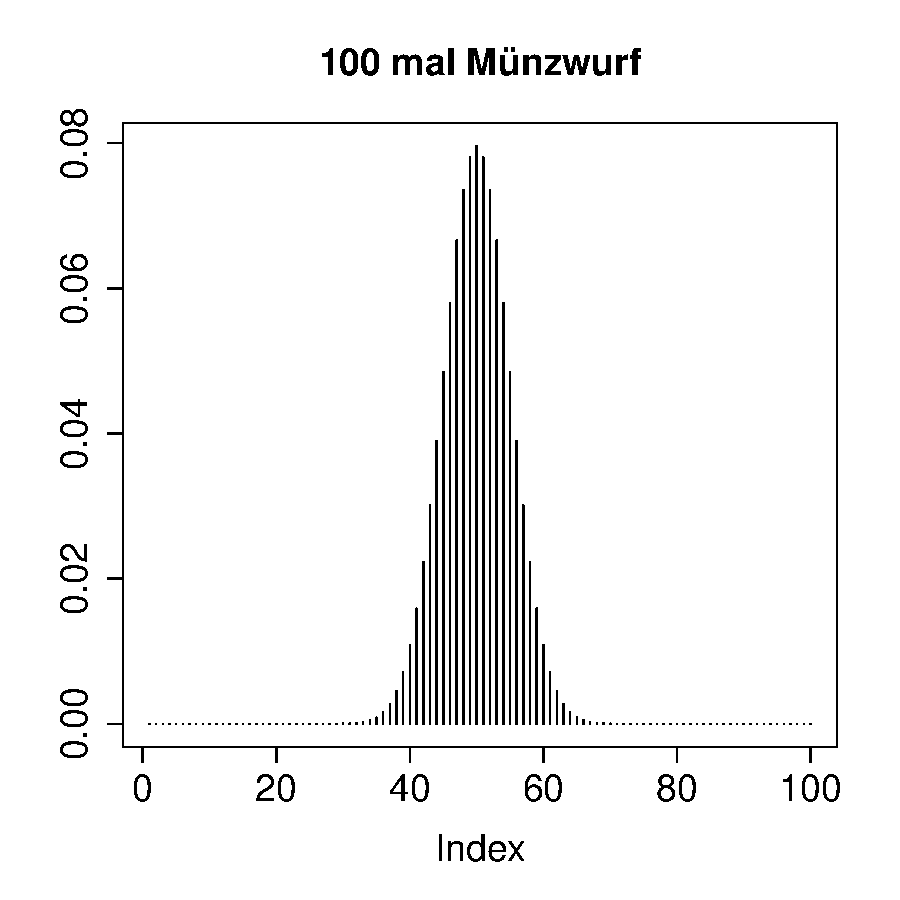
\includegraphics{verteilungen-017}
\caption{Verteilung für 100 Versuche}
\end{subfigure}
\begin{subfigure}[b]{0.48\textwidth}
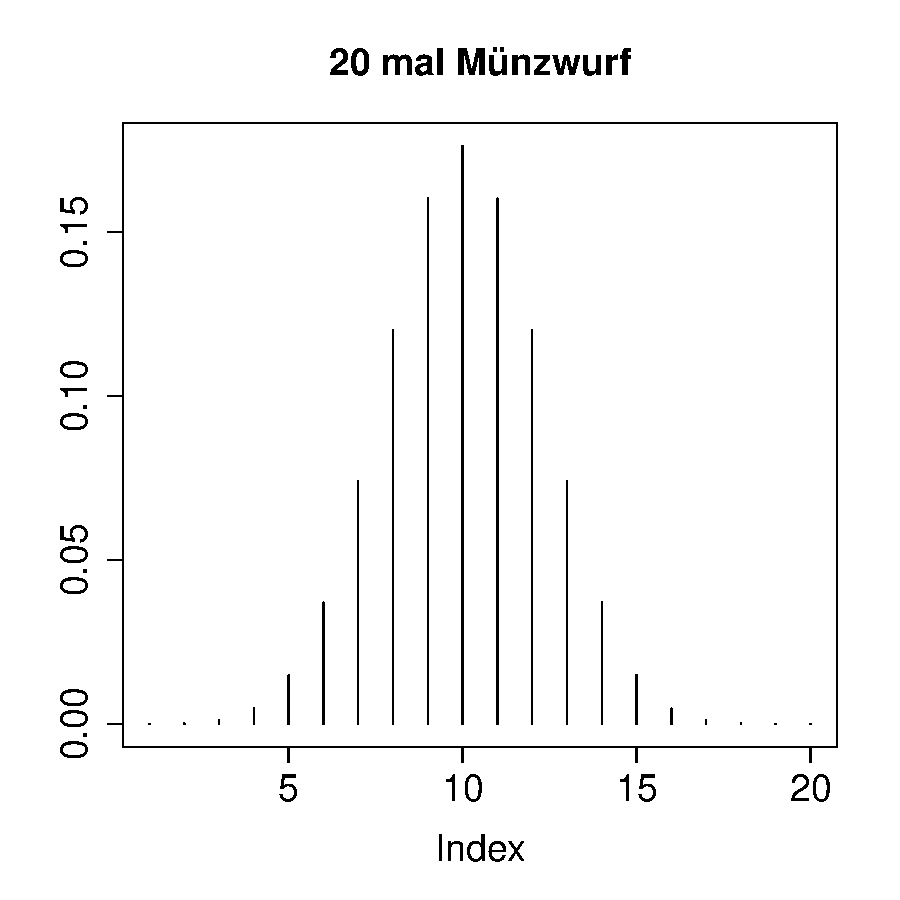
\includegraphics{verteilungen-018}
\caption{Verteilung für 20 Versuche}
\end{subfigure}
\caption{Wahrscheinlichkeitsverteilung beim Münzwurf}
\end{figure}

\clearpage
\newpage
\section{Poissonverteilung}

\subsection{Verwendung in R}
\lstinline{R} stellt grundsätzlich vier Funktionen für die 
Poissonverteilung zur Verfügung. 
\begin{itemize}
	\item \lstinline{dpois()} \hfill{} 
		(\emph{Wahrscheinlichkeitsverteilung})
	\item \lstinline{pois()} \hfill{}
		(\emph{kumulative Wahrscheinlichkeit})
	\item \lstinline{qpois()} \hfill{}
		(\emph{Verteilung der Quantile})
	\item \lstinline{rpois()} \hfill{}
		(\emph{Zufallszahlen})
\end{itemize}





\begin{figure}[h!]
\centering
\begin{subfigure}[b]{0.48\textwidth}
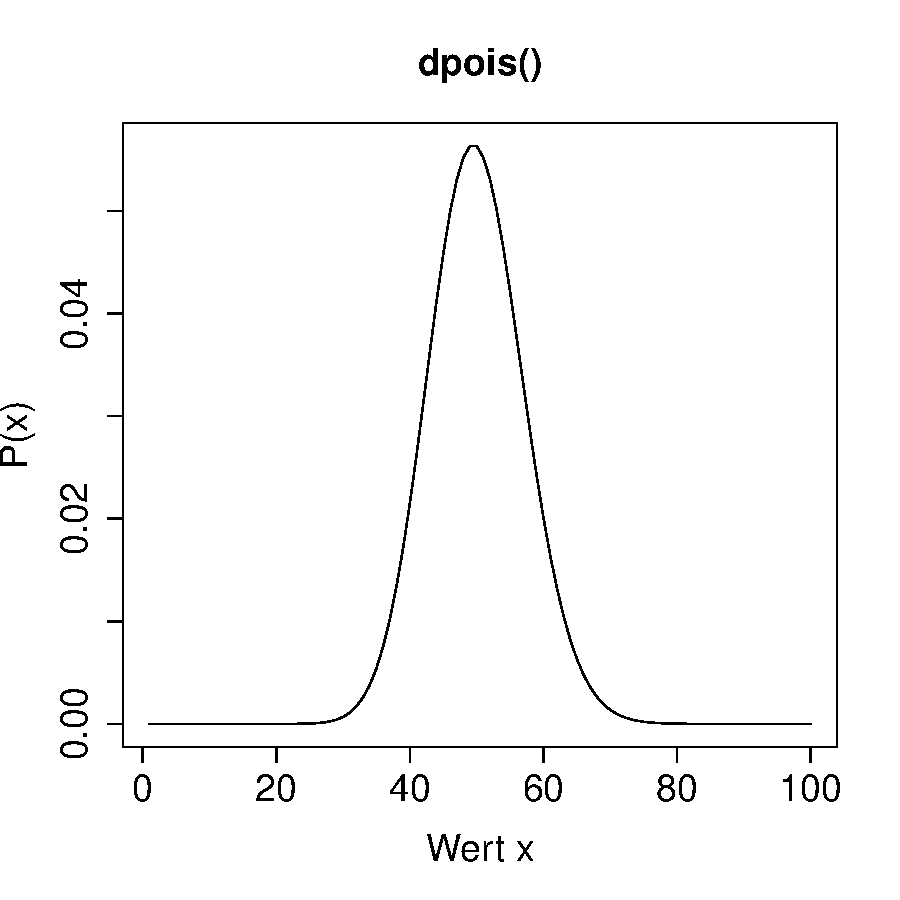
\includegraphics{verteilungen-023}
\caption{W.-Verteilung}
\end{subfigure}
\begin{subfigure}[b]{0.48\textwidth}
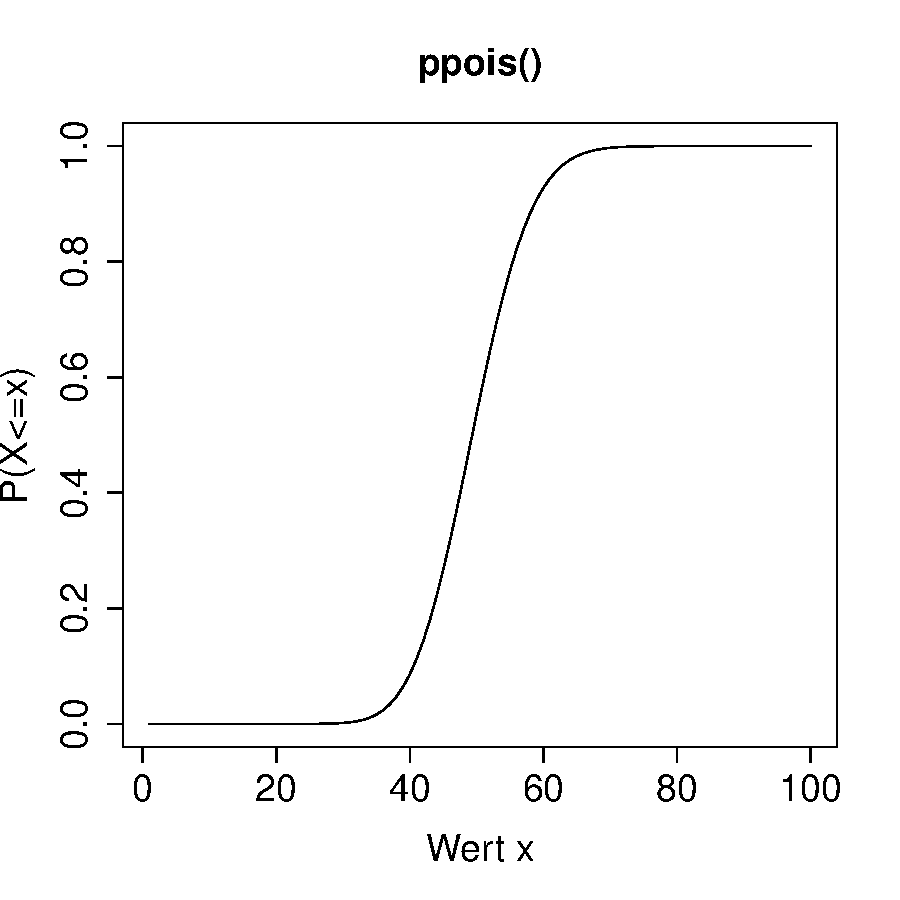
\includegraphics{verteilungen-024}
\caption{kumulative Wahrscheinlichkeit}
\end{subfigure}

\begin{subfigure}[b]{0.48\textwidth}
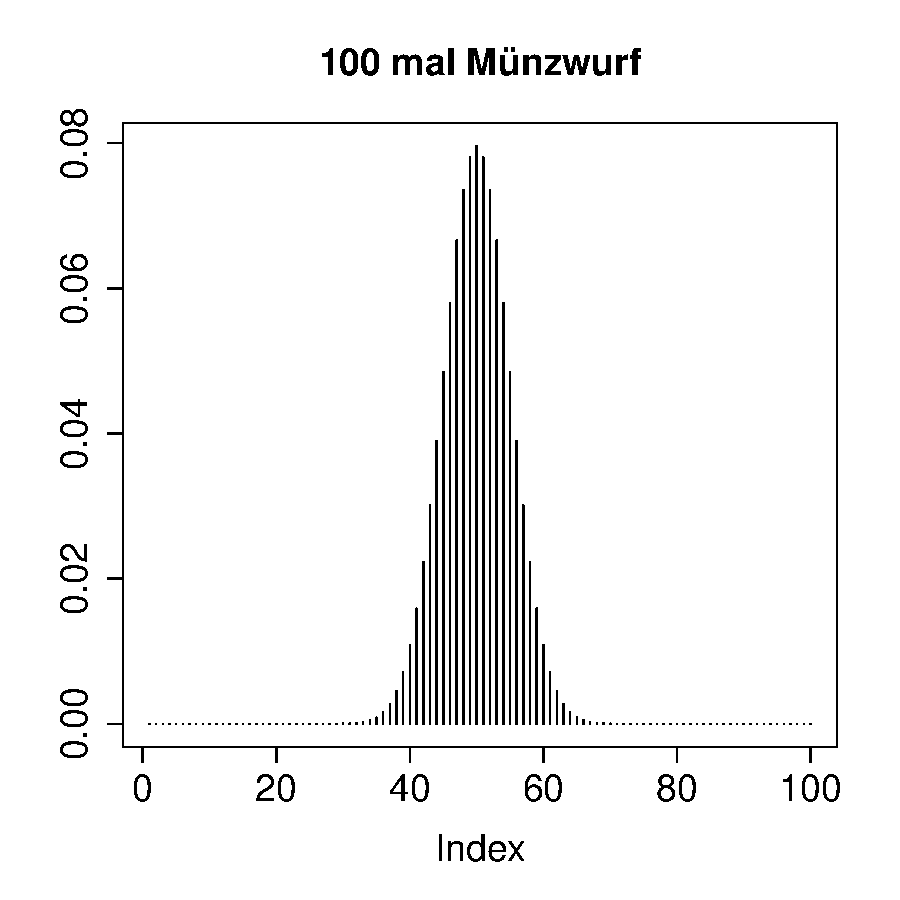
\includegraphics{verteilungen-025}
\caption{Quantile}
\end{subfigure}
\begin{subfigure}[b]{0.48\textwidth}
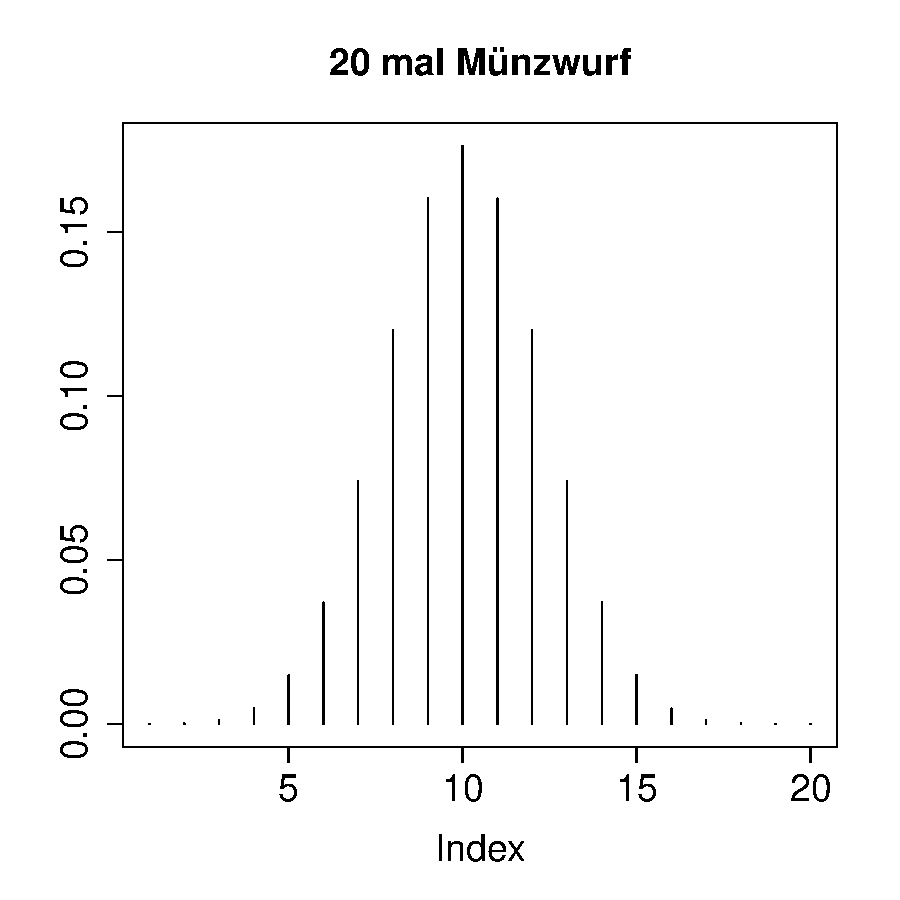
\includegraphics{verteilungen-026}
\caption{Zufallszahlen}
\end{subfigure}
\caption{Poissonverteilung ($\lambda=50$)}
\end{figure}

\section{Erwartungswert}
Der Erwartungswert einer diskreten Verteilung gibt jene Zahl an,
welche die Zufallsvariable im \emph{Mittel} annimmt. Sie beschreibt
quasi den mittleren Wert der Verteilung.

Für diskrete Wahrscheinlichkeitsverteilungen gilt, dass der 
Erwartungswert der Summe von Produkten aus Wahrscheinlichkeit und
Wert der Zufallsvariable entspricht. 
\[ \mu = E(X) = \sum x \cdot P(X=x) \]
$P(X=x)$ bedeutet \emph{Wahrscheinlichkeit, dass die Zufallsvariable $X$ 
genau $x$ ist}.


\section{Varianz}
Die Varianz einer Wahrscheinlichkeitsverteilung gibt ein Mass an für 
die Streuung der Warscheinlichkeiten um den Erwartungswert.

Die Varianz wird analog zum Erwartungswert ermittelt, wobei der Wert
der Zufallsvariable $x$ ersetzt wird durch das Quadrat der Abweichung
von Zufallsvariable und Erwartungswert $(x-\mu)^2$
\[ \begin{array}{l c l}
	Var(X) 
		& = 
		& E(X-\mu)^2 \\
	& &  \\
	Var(X)
		& = 
		& \sum \left( (x-\mu)^2 \cdot P(X=x) \right)
\end{array} \]

\section{Standardabweichung}
Die Standardabweichung einer Wahrscheinlichkeitsverteilung 
ist wie die Varianz ein Mass für die Streuung. Sie 
wird anhand der Varianz ermittelt mit dem Zusammenhang, dass die 
Standardabweichung der Quadratwurzel der Varianz entspricht.
\[ \begin{array}{l c l} 
	\sigma 
		& = 
		& \sqrt{Var(X)} \\
	& & \\
	\sigma
		& =
		& \sqrt{E(X-\mu)^2} \\
	& & \\
	\sigma
		& =
		& \sqrt{\sum \left( (x-\mu)^2 \cdot P(X=x) \right)}
\end{array} \]

\section{Zusammenfassung}

\begin{table}[h!]
	\centering
	\begin{tabular}{l c c}
		Verteilung
			& $E(X)$
			& $V(X)$ \\
		\hline
		& & \\
		$X \sim Hyp(n,r,s)$
			& $n \cdot \left(\frac{r}{r+s}\right)$
			& $n \cdot \left( 
				\frac{r}{r+s}
				\right) 
			\left( 
				1 - \frac{r}{r+s}
			\right)
			\left(
				\frac{(r+s)-n}{(r+s)-1}
			\right)$ \\
		& & \\
		$X \sim Bin(n,p)$
			& $n \cdot p$
			& $n \cdot p \cdot (1-p)$ \\
		& & \\
		$X \sim Pois(\lambda)$
			& $\lambda$
			& $\lambda$
	\end{tabular}
\end{table}

